\section{Устройство памяти}
\begin{enumerate}
 \item Память состоит из адресуемых ячеек (размером 1 -- 128 бит). Ячейки в основном организованы по 8 бит и свой собственный адрес имеет только каждый восьмой бит.
 \item Ячейки состоят из запоминающих электрических элементов. Это может быть конденсатор, транзистор, попупроводниковый материал и т.п., умеющий хранить два состояния (заряжен или разряжен -- конденсатор, находится в проводящем или непроводящем состоянии -- транзистор, имеет высокое или низкое удельное сопротивление -- попупроводниковый материал). Есть так же элементы, умеющие хранить три состояния, но эти три состояния сложнее считывать.
 \item Электрический элемент может находиться в одном из двух устойчивых состояний (для хранения 1 бита):
 \begin{itemize}
   \item конденсатор заряжен/разряжен;
   \item транзистор в проводящем/непроводящем состоянии;
   \item полупроводниковый материал имеет высокое/низкое сопротивление.
 \end{itemize}
\end{enumerate}
Одно из таких физических состояний создает высокий уровень выходного напряжения элемента памяти, а другое -- низкий. В элементах памяти ряда микроЭВМ это электрические напряжения порядка 4В и 0В соответственно, причем первое обычно принимается за двоичную единицу, а второе -- за двоичный нуль (возможно и обратное кодирование.)
\begin{figure}[h]
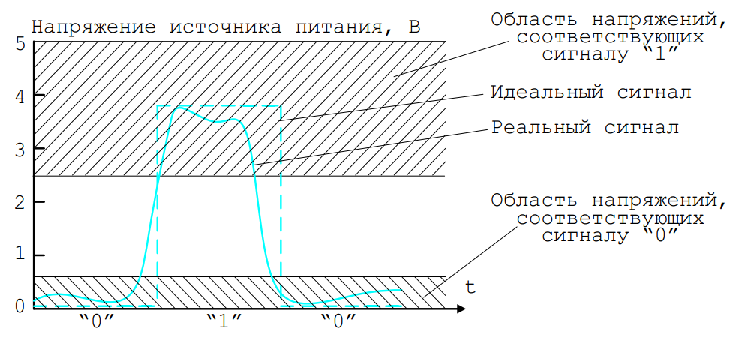
\includegraphics[width=\textwidth]{10_1}
\end{figure}
\\На рисунке показан выходной сигнал элемента памяти (например, одного разряда регистра) при изменении его состояний (при переключениях) под воздействием некоторого входного сигнала. Хотя переход от 0 к 1 и от 1 к 0 происходит не мгновенно, однако в определенные моменты времени этот сигнал достигает значений, которые воспринимаются элементами ЭВМ как 0 или 1. Если сигнал попадает в незаштрихованную область (между 0,5В и 2,5В) то сигнал не распознается.
\\
\\\textbf{Запоминающим элементом} называется элемент, который способен принимать и хранить код двоичной цифры (исходные значения некоторых величин, промежуточные значения обработки и окончательные результаты вычислений). Элементы памяти могут запоминать и сохранять исходные значения некоторых величин, промежуточные значения обработки и окончательные результаты вычислений. Только запоминающие элементы в схемах ЭВМ позволяют проводить обработку информации с учетом ее развития.
\\\textbf{Триггер} -- элементарный цифровой автомат, обладающий способностью длительно находиться в одном из двух устойчивых состояний и чередовать их под воздействием внешних сигналов. Состояние $0$ на выходе $Q$ соответствует выключенному состоянию, а $Q = 1$ -- включенному. Триггеры осуществляют запоминание информации и остаются в заданном состоянии после прекращения действия переключающих сигналов. Они широко применяются широко применяются при цифровой обработке информации.
\\По способу организации логических связей, определяющие особенности функционирования, различают триггеры:
\begin{itemize}
  \item \textbf{RS--триггер} -- меняет свое состояние в зависимости от того, на какой из входов была подана единица. При подаче сигнала на вход $S$ (\emph{Set}) на выходе устанавливается единица. При подаче сигнала на вход $R$ (\emph{Reset}) сигнал на выходе пропадает.
  \item  \textbf{D--триггер} (\emph{Delay} или \emph{Data}) -- запоминает (задерживает) состояние входа на один такт. При кратковременной подаче сигнала на $C$ (\emph{Clock}) (обычно, с тактового генератора), запоминает сигнал на входе $D$ (\emph{Data}) и выдает его на выход до следующей итерации.
  \item \textbf{Т--триггер} (\emph{Toggle}) -- при подаче сигнала на вход, меняет сигнал на выходе на противоположный.
  \item \textbf{JK--триггер} -- аналогичен $RS$--триггеру ($J$ (\emph{Jump}) = $Set$, $K$ (\emph{Kill}) = $Reset$), с одним лишь исключением: при подаче единицы на оба входа, состояние выхода изменяется на противоположное.
\end{itemize}
Из них JK триггер называется универсальным, так как из него можно получить все остальные виды триггеров.
\begin{figure}[!h]
\begin{minipage}{5cm}
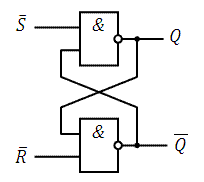
\includegraphics[width=5cm]{10_2}
\caption{Асинхронный RS--триггер на элементах 2И--НЕ (IEC)}
\end{minipage}
\hfill
\begin{minipage}{5cm}
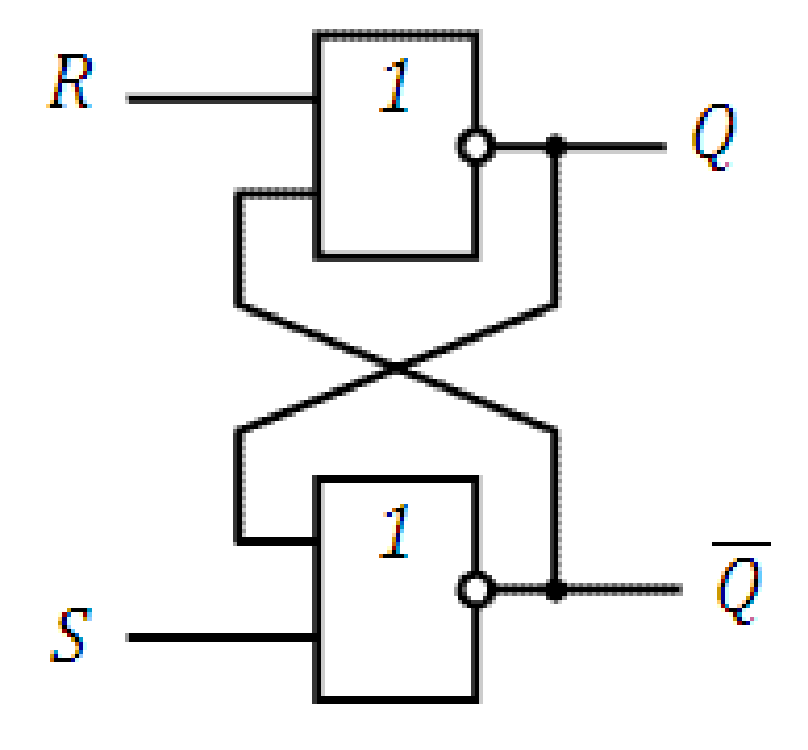
\includegraphics[width=4.7cm]{10_3}
\caption{Асинхронный RS--триггер на элементах 2ИЛИ--НЕ (IEC)}
\label{tag:RS_NOR}
\end{minipage}
\end{figure}

\textbf{Регистры} -- это узлы ЭВМ, служащие для хранения информации в виде машинных слов или его частей, а так же для выполнения над словами некоторых логических преобразований.
Регистры способны выполнять следующие операции:
\begin{itemize}
  \item установка регистра в состояние 0 или 1 (на всех выходах);
  \item прием и хранение в регистре n разрядного слова;
  \item сдвиг хранимого в регистре двоичного кода слова вправо или влево на заданное значение разрядов;
  \item преобразование кода хранимого слова в последовательный, и наоборот, при приеме или при выдачи двоичных данных;
  \item поразрядные логические операции.
\end{itemize}
\textbf{Счетчики} -- узлы ЭВМ, которые осуществляют счет и хранение кода числа подсчитанных сигналов.Они представляют собой цифровые автоматы Мура, в которых новое состояние счетчика определяется его предыдущим состоянием и состоянием логической переменной на входе.
\\Внутреннее состояние счетчиков характеризуется коэффициентом пересчета К, определяющим число его устойчивых состояний. Основными параметрами являются разрешающая способность (минимальное время между двумя сигналами, которые надежно фиксируются) или максимальное быстродействие и информационная емкость.
\\\textbf{Дешифратор (избирательная схема)} -- это узел ЭВМ, в котором каждой комбинации входных сигналов соответствует наличие сигнала на одной вполне определенной шине на выходе (комбинационное устройство). Дешифраторы широко используются для преобразования двоичных кодов в управляющие сигналы для различных устройств ЭВМ.
\\\textbf{Шифратор (кодер)} -- это узел ЭВМ, преобразующий унитарный код в некоторый позиционный код. Если выходной код является двоичным позиционным, то шифратор называется двоичным. С помощью шифраторов возможно преобразование цифр десятичных чисел в двоичное представление с использованием любого другого двоично--десятичного кода.
\\\textbf{Преобразователи кодов} -- это узлы ЭВМ, предназначенные для кодирования чисел. В число преобразователей кодов входят: двоично--десятичные преобразователи, преобразователи цифровой индикации, преобразователи прямого кода двоичных чисел в обратный или дополнительный код и т. д.
\\\textbf{Мультиплексоры} -- это узлы, преобразующие параллельные цифровые коды в последовательные. В этом устройстве выход соединяется с одним из входов в зависимости от значения адресных входов. Мультиплексоры широко используются для синтеза комбинационных устройств, так как это способствует значительному уменьшению числа используемых микросхем.
\\\textbf{Демультиплексоры} -- это узлы, преобразующие информацию из последовательной формы в параллельную. Информационный вход D подключается к одному из выходов Qi определяемый адресными сигналами A0 и A1.
\begin{figure}[!h]
\begin{minipage}[c]{6cm}
\center{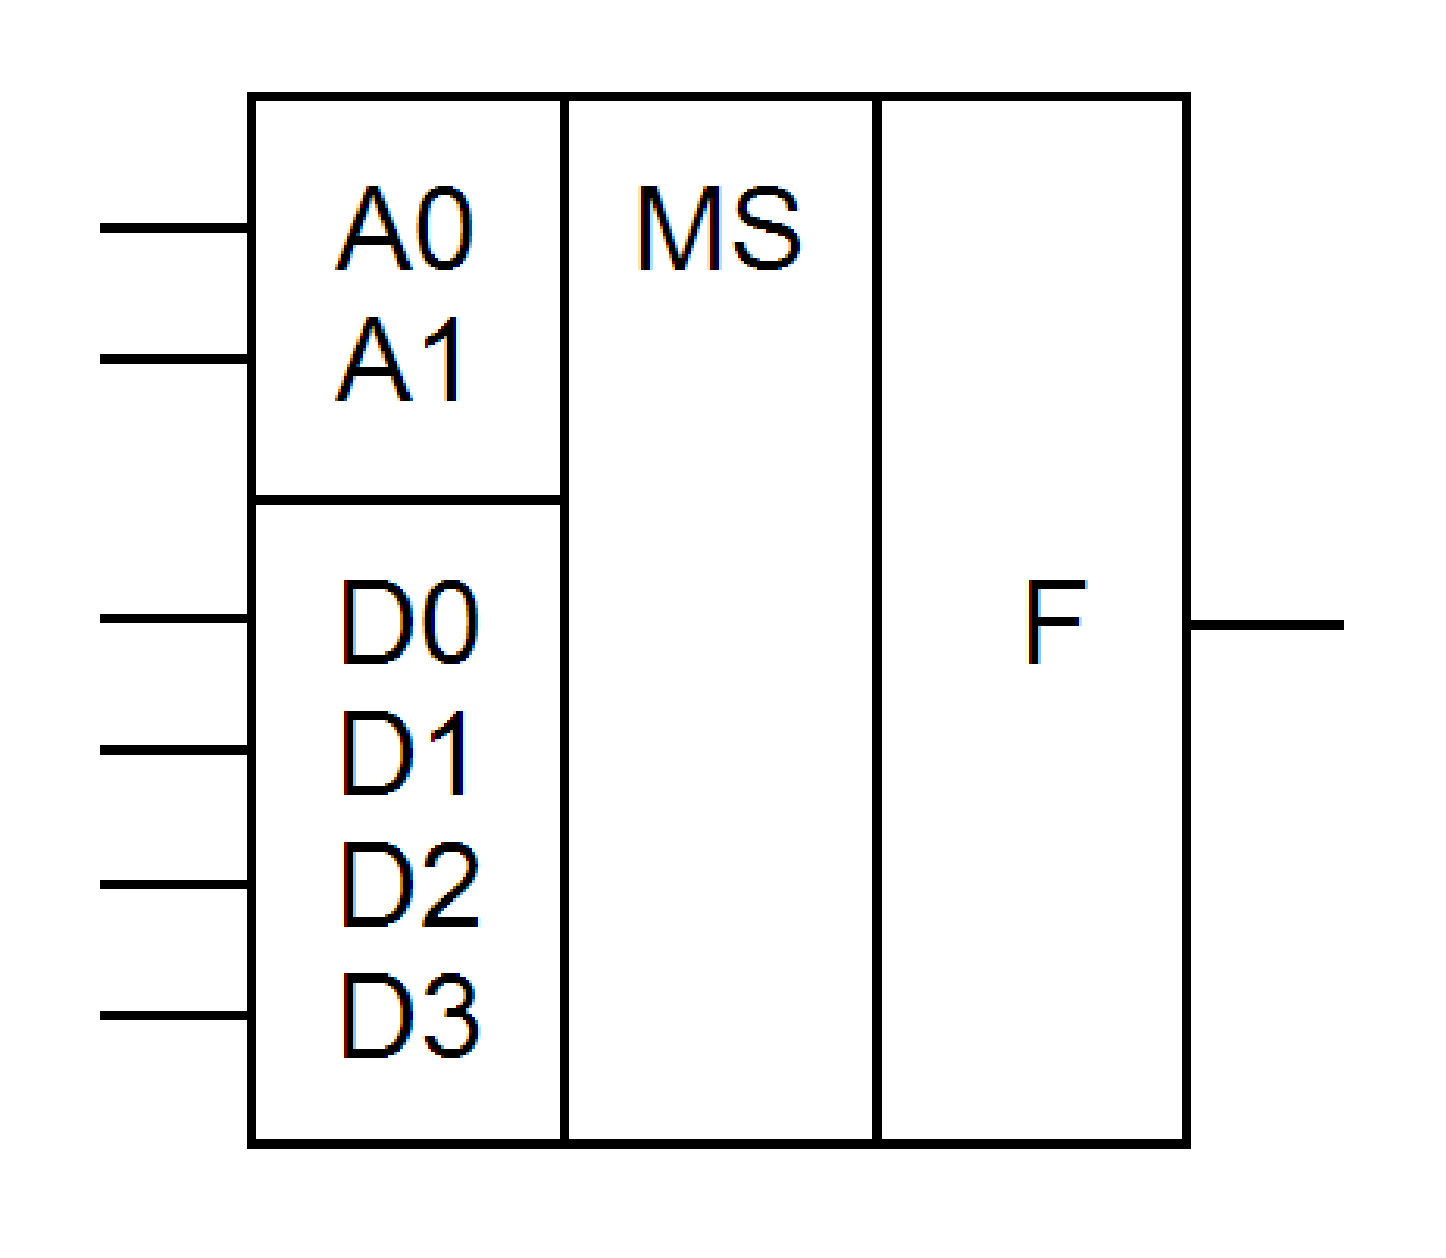
\includegraphics[width=3.5cm]{10_4}}
\caption{Мультиплексор}
\end{minipage}
\hfill
\begin{minipage}[c]{6cm}
\center{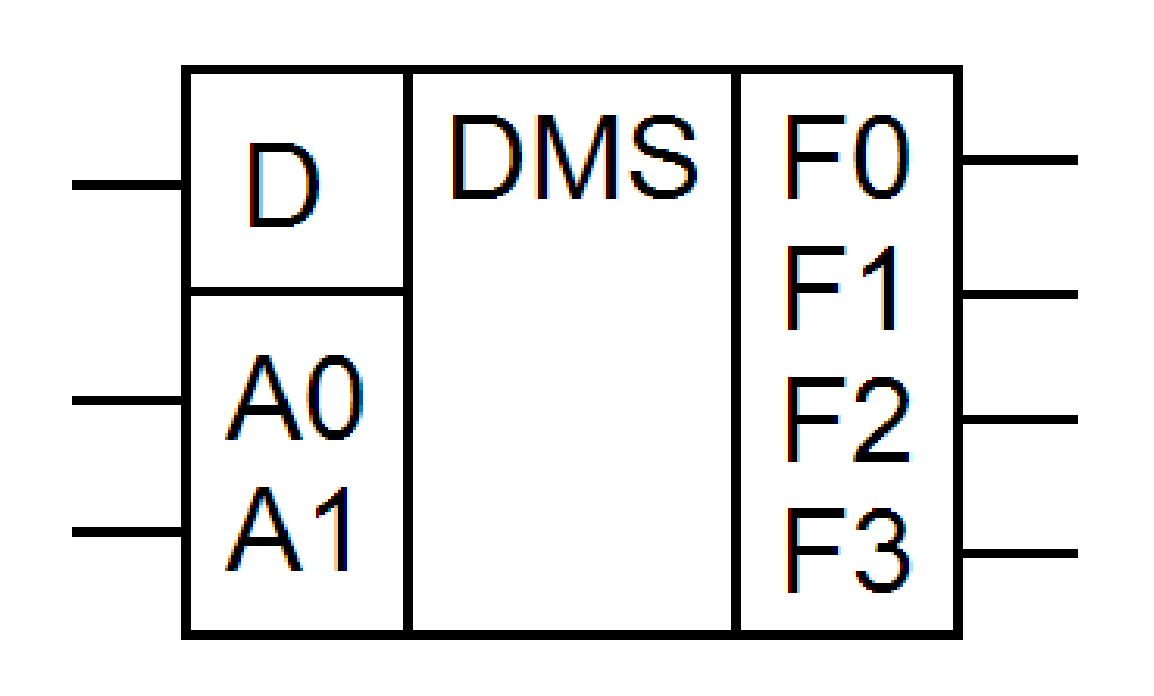
\includegraphics[width=3.5cm]{10_5}}
\caption{Демультиплексор}
\end{minipage}
\end{figure}

\textbf{Сумматор} -- это узел, в котором выполняется арифметическая операция суммирования цифровых кодов двух двоичных чисел.
\\Используя одноразрядные сумматоры можно построить многоразрядные сумматоры.
\\\textbf{Шина} -- набор коммуникационных линий, каждая из которых способная передавать сигналы, представляющие двоичные цифры 0 и 1. 
\\Электрическая цепь, соединяющая регистр с другим регистром или иным устройством ЭВМ, называется \textbf{шиной (bus)}. \emph{Шина} состоит из параллельных проводов, каждый из которых предназначен для передачи соответствующего бита регистра. Два 8--битовых регистра соединяются между собой шиной из восьми проводов. Про такую шину говорят, что ее ширина равна 8. В действительности шина обычно содержит несколько дополнительных проводов, используемых для передачи сигналов синхронизации и управления, однако подобный анализ структуры шин нас пока не интересует.
\section{Характеристики систем памяти}
\begin{enumerate}
  \item\textbf{ Место расположения:}
  \begin{itemize}
    \item \emph{Процессорная}, то есть на общем кристалле с центральным процессором (ЦП) (регистры, кэш--память 1--го уровня);
    \item \emph{Внутренняя}, то есть на системной плате (основная память (ОП), кэш--память 2--го и последующего уровней);
    \item \emph{Внешняя} (медленные запоминающие устройства (ЗУ) большой ёмкости).
  \end{itemize}
  \item \textbf{Емкость ЗУ} -- число бит/байт, которое можно хранить на ЗУ.
  \item \textbf{Единица пересылки.} Для ОП единица пересылки определяется шириной шины данных, то есть количество бит, передаваемых по линиям шины параллельно. Обычно равна длине слова.
  \item \textbf{Метод доступа к данным:}
  \begin{itemize}
    \item \emph{Последовательный доступ} -- ЗУ ориентировано на хранение информации в виде последовательности блоков, называемых записями. Для доступа к нужному элементу необходимо прочитать все предшествующие блоки (ЗУ на магнитной ленте);
    \item \emph{Прямой доступ} -- каждая запись имеет уникальный адрес, отражающий ее физическое размещение на носителе информации. Обращение определяется как адресный доступ к началу записи плюс последующий последовательный доступ к определённой информации внутри записи (магнитные диски);
    \item \emph{Произвольный доступ} -- каждая ячейка памяти имеет уникальный физический адрес. Обращение к любой ячейке занимает одно и то же время и может водиться в произвольной очередности (ОП);
    \item \emph{Ассоциативный доступ} -- позволяет выполнять поиск ячеек, содержащих такую информацию, в которой значение отдельных бит совпадает с состоянием одноименных битов в заданном образце. Сравнение осуществляется параллельно для всех ячеек памяти, независимо от ее емкости (кэш--память).
  \end{itemize}
  \item \textbf{Быстродействие} -- один из важнейших показателей:
  \begin{itemize}
    \item \emph{Время доступа ($\mbox{Т}_{\mbox{д}}$)} -- интервал времени от момента поступления адреса до момента, когда данные заносятся в память или становятся доступными.
    \item \emph{Длительность цикла памяти или период обращения ($\mbox{Т}_{\mbox{ц}}$)} -- понятие применяется к памяти с произвольным доступом, для которой оно означает минимальное время между двумя последовательными обращениями к памяти. Период обращения включает в себя время доступа плюс некоторое дополнительное время.
    \item \emph{Скорость передачи} -- скорость, с которой данные могут передаваться в память или из нее.
  \end{itemize}
  \item \textbf{Физический тип}
  \begin{itemize}
    \item Полупроводниковая память;
    \item Память с магнитным носителем информации (используемая в магнитных лентах и дисках);
    \item Память с оптическим носителем (оптические диски);
  \end{itemize}
  \item \textbf{Физические особенности} (например, энергозависимость).
  \item \textbf{Стоимость} -- стоимость хранения одного бита информации.
\end{enumerate}
\section{Иерархия памяти}
\begin{figure}[!h]
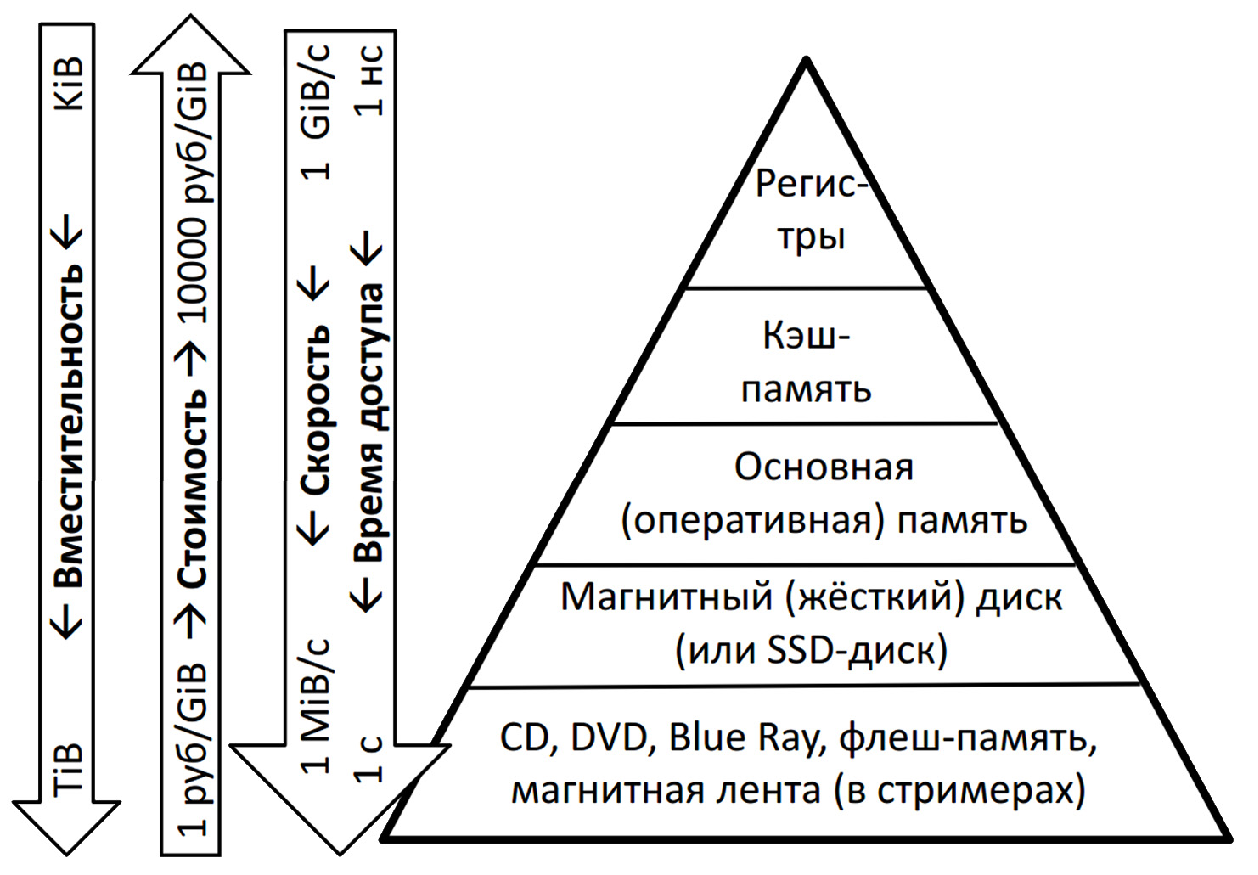
\includegraphics[width=9cm]{10_6}
\end{figure}
Чем меньше время доступа, тем выше стоимость хранения бита. Чем больше емкость, тем ниже стоимость хранения бита, но больше время доступа.

\section{Физическое устройство памяти}
\subsection{Кэш--память}
\begin{wrapfigure}[7]{l}{1.7cm}
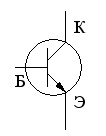
\includegraphics[width=1.7cm]{10_7_(1)}
\end{wrapfigure}
Рассмотрим биполярный \emph{n--p--n} транзистор: К -- коллектор, Б -- база, Э -- эмиттер. На коллектор подано напряжение. Если на базу подать напряжение -- транзистор откроется и ток с коллектора пойдет на эмиттер.
\\Небольшая особенность -- напряжение на базе должно быть выше, чем на коллекторе (на сколько -- зависит от конкретного транзистора, обычно немного. Например, 5В на коллекторе, 6В на базе).
\\
\\Теперь рассмотрим следующую схему:
\\
\begin{minipage}[l]{5cm}
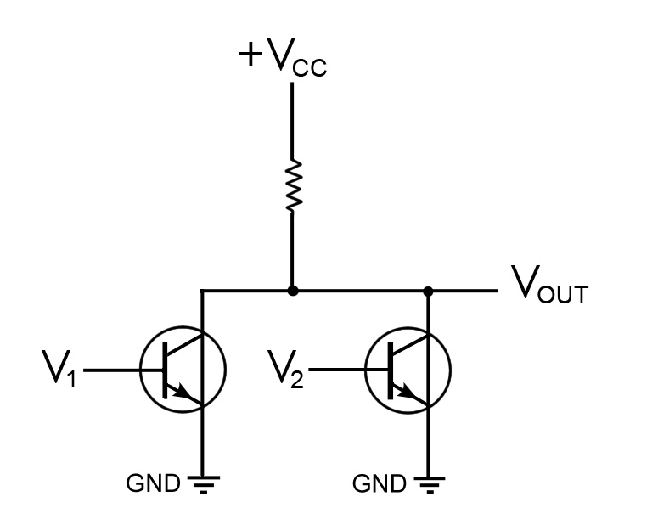
\includegraphics[width=5cm]{10_7}
\end{minipage}
\begin{minipage}[l]{7cm}
$V_{CC}$ -- линия питания устройства (например 5В).
\\$GND$ -- линия 0В.
\\Если оба транзистора закрыты (на базу не подается напряжение, $V_1$ и $V_2$ равны 0), то ток уходит напрямую с $V_{CC}$ на $V_{OUT}$. В результате получается логическая единица.
\\Если подать напряжение хотя бы на один транзистор ($V_1$ или $V_2$), то ток с $V_{CC}$ будет уходить через транзистор в $GND$ и в $V_{OUT}$ не пойдет. В результате получается логический нуль.
\end{minipage}
\\
\\Так как напряжение на базе должно быть выше, чем на коллекторе (в данном случае, на линии питания $V_{CC}$), а повышенное взять неоткуда, то имеющееся напряжение на $V_{CC}$ занижается с помощью резистора и получается 5В на базе и чуть меньше на коллекторе.
\\
\\Получается, что данная схема реализует логическую функцию ИЛИ--НЕ (ANSI) (также известную как стрелка Пирса) (где $A$ и $B$ соответственно $V_1$ и $V_2$):

\begin{minipage}[l]{4cm}
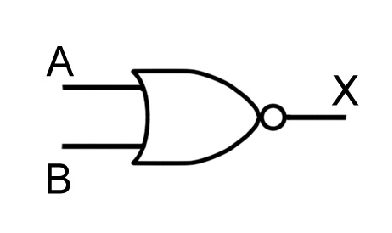
\includegraphics[width=2.8cm]{10_8}
\end{minipage}
\\
\\Таблица истинности для ИЛИ--НЕ:
\begin{table}[!h]
\begin{tabular}{|c|c|c|}
\hline
A & B & X \\
\hline
 0 & 0 & 1 \\
 0 & 1 & 0 \\
 1 & 0 & 0 \\
 1 & 1 & 0 \\
\hline
\end{tabular}
\end{table}
\\Объединим два элемента ИЛИ--НЕ обратной связью.
\begin{wrapfigure}[10]{l}{3.8cm}
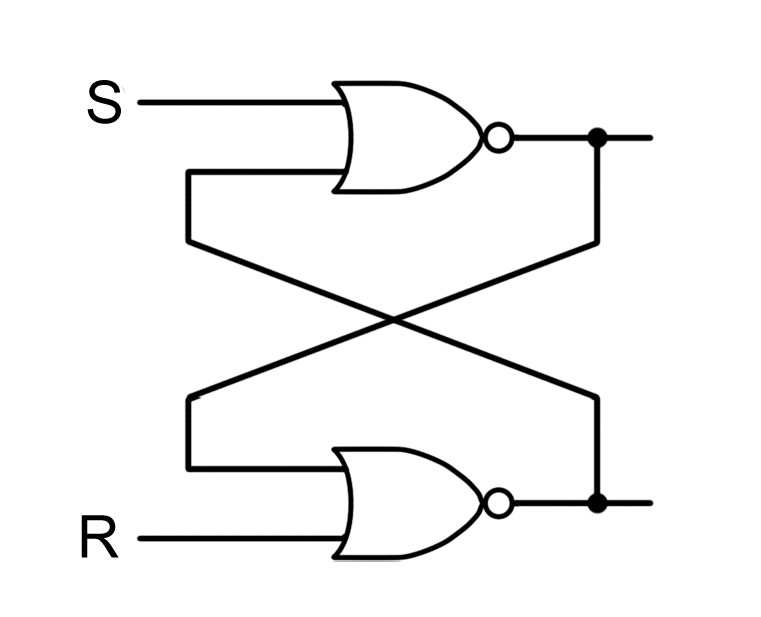
\includegraphics[width=3.8cm]{10_9}
\end{wrapfigure}
Выход одного элемента ИЛИ--НЕ поступает на вход другого. Получилась самая простая память для хранения 1 бита, использующая 4 транзистора.
\\В данном случае, изображен асинхронный RS--триггер (изображен на рисунке \ref{tag:RS_NOR}). Также, память может состоять и из других триггеров.
\\При подаче единицы на вход $S$ выходное состояние становится равным логической единице. А при подаче единицы на вход $R$ выходное состояние становится равным логическому нулю. Если на оба входа $R$ и $S$ одновременно поданы логические единицы, оба выхода переходят в состояние логического нуля, которое является неустойчивым и переходит в одно из устойчивых состояний при снятии управляющего сигнала с одного из входов, иначе говоря, в ячейку может записаться любое значение.
\subsection{Оперативная память}
\begin{wrapfigure}[10]{l}{4cm}
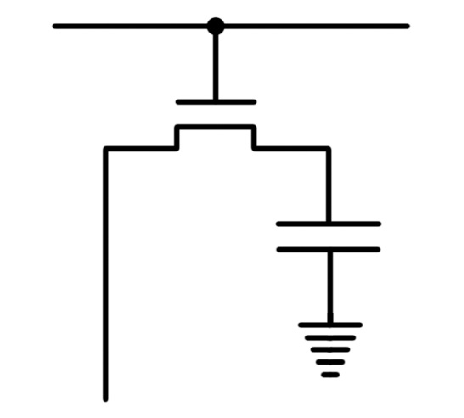
\includegraphics[width=4cm]{10_10}
\end{wrapfigure}
В отличие от кэш--памяти, оперативная память устроена намного проще. Она устроена из 1 конденсатора и 1 транзистора, что дешево и занимает мало места. Один конденсатор легче воспринимать как память (конденсатор разряжен -- 0, заряжен -- 1). Транзистор нужен с одной целью -- чтобы не разряжать постоянно конденсатор. Конденсатор необходимо периодически подзаряжать, а заряжается и разряжается он медленно. Переключить транзистор быстрее чем, зарядить или разрядить конденсатор.
\\Если на базу подано напряжение, транзистор открыт, мы можем считать значение -- 1. Если напряжения нет, значение не считывается, записывается 0.
\section{Локальность памяти}
\subsection{Пространственная локальность памяти}
С очень высокой вероятностью адрес очередной команды программы либо следует непосредственно за адресом, по которому была считана текущая команда, либо расположен вблизи него. Такое расположение адресов называется \textbf{пространственной локальностью программы}.
\\Обрабатываемые данные, как правило, структурированы, и такие структуры обычно хранятся в последовательных ячейках памяти. Такая особенность программ называется \textbf{пространственной локальностью данных}.
\subsection{Временн\'ая локальность памяти}
Кроме того, программы содержат множество небольших циклов и подпрограмм. Это означает, что небольшие наборы команд могут многократно
повторяться в течение некоторого интервала времени, то есть имеет место \textbf{временная локальность}.
\\Все три вида локальности объединяет понятие \textbf{локальность по обращению}. Принцип локальности часто облекают в численную форму и представляют в виде так называемого правила "90/10": 90 \%
 времени работы программы связано с доступом к 10\%
  адресного пространства этой программы.
  \subsection{Применение локальности памяти}
 
 Рассмотренные принципы локальности не являются просто любопытным наблюдением. Их использовуют для устранения проблемы узкого места архитектур фон Неймана — шины взаимодействия между процессором и памятью.
 \\
 \\ Память, как правило, работает на меньшей частоте и с меньшей скоростью чем процессор, но программа достаточно часто обращается к памяти. Это приводит к тому, что скорость работы программы и скорость работы компьютера определяется не скоростью работы процессора, а скоростью работы медленной оперативной памяти.
\\Чтобы устранить эту проблему обычно используют кэш, и эффект от него достаточно ощутим: сильный выигрыш в производительности.
Но почему же тогда вместо медленной оперативной памяти не использовать быструю кэш--память? Рассмотрим пример.
\\
\\Так как мы хотим полностью заменить оперативную памать на кэш, то стоимость компьютера увеличится в сто или даже в тысячу раз (оперативной памяти обычно устанавливают гигабайты, а кэш--память измеряется всего лишь мегабайтами). 
\\Чтобы посчитать к какому эффекту это приведёт, будем использовать принцип Парето (\emph{`20\% усилий дают 80\% результата, а остальные 80\% усилий — лишь 20\% результата`}), в соответствии с которым, из--за локальности обращений, 80\% таких обращений попадают в кэш. То есть, при первом обращении большой объем данных приходится копировать из оперативной памяти, что достаточно медленно. Зато далее, в процессе работы программы, с очень высокой вероятностью (в нашем случае – 80\%) при записи/чтении очередной порции данных из памяти мы можем взять её в готовом виде из кэш--памяти. Будем считать, что кэш--память работает в 10 раз быстрее оперативной памяти.
\\Посчитаем, сколько времени понадобится, чтобы выполнить N операций записи или чтения. 
\\Оказывается, что в компьютере, где используется медленная оперативная память, то есть до гипотетической модернизации, время выполнения программы будет равно 2,8N (условно измеряемое в наносекундах).
После замены оперативной памяти на кэш--память, все обращения будут происходить со скоростью кэша, следовательно, общее время сократится до N.
\\
\\
Увидев эти цифры можно сделать любопытный вывод. Мы потратили деньги для того, чтобы ускорить работу памяти в 10 раз, но при этом 10--кратное ускорение памяти привело лишь к трехкратному увеличению производительности. 
В этом и состоит эффект кэширования: вовсе не обязательно устанавливать в компьютере дорогостоящую быструю память, можно обойтись несколькими уровнями кэша, каждый из которых чуть быстрее (а желательно – на порядок быстрее) предыдущего. Это позволит очень эффективно бороться с узким местом принстонской архитектуры.

\section{Порядок хранения байт в памяти}
Существует несколько способов хранения байт в памяти:
\begin{itemize}
  \item \textbf{От старшего к младшему} (англ. \emph{big--endian}): $A_n,\dots,A_0$ запись начинается со старшего и заканчивается младшим. Этот порядок является стандартным для протоколов TCP/IP, он используется в заголовках пакетов данных и во многих протоколах более высокого уровня, разработанных для использования поверх TCP/IP. Поэтому, порядок байтов от старшего к младшему часто называют сетевым порядком байтов.
  \item \textbf{От младшего к старшему} (англ. \emph{little--endian}): $A_0,\dots,A_n$ запись начинается с младшего и заканчивается старшим. Этот порядок записи принят в памяти персональных компьютеров с x86--процессорами, в связи с чем иногда его называют интеловский порядок байт (по названию фирмы--создателя архитектуры x86).
  \item \textbf{Переключаемый порядок} (англ. \emph{bi--endian}). Многие процессоры могут работать и в порядке от младшего к старшему, и в обратном. Обычно порядок байтов выбирается программно во время инициализации операционной системы, но может быть выбран и аппаратно перемычками на материнской плате. В этом случае правильнее говорить о порядке байтов операционной системы.
  \item \textbf{Смешанный порядок} (англ. \emph{middle--endian}) иногда используется при работе с числами, длина которых превышает машинное слово. Число представляется последовательностью машинных слов, которые записываются в формате, естественном для данной архитектуры, но сами слова следуют в обратном порядке.
\end{itemize}
\begin{figure}[h]
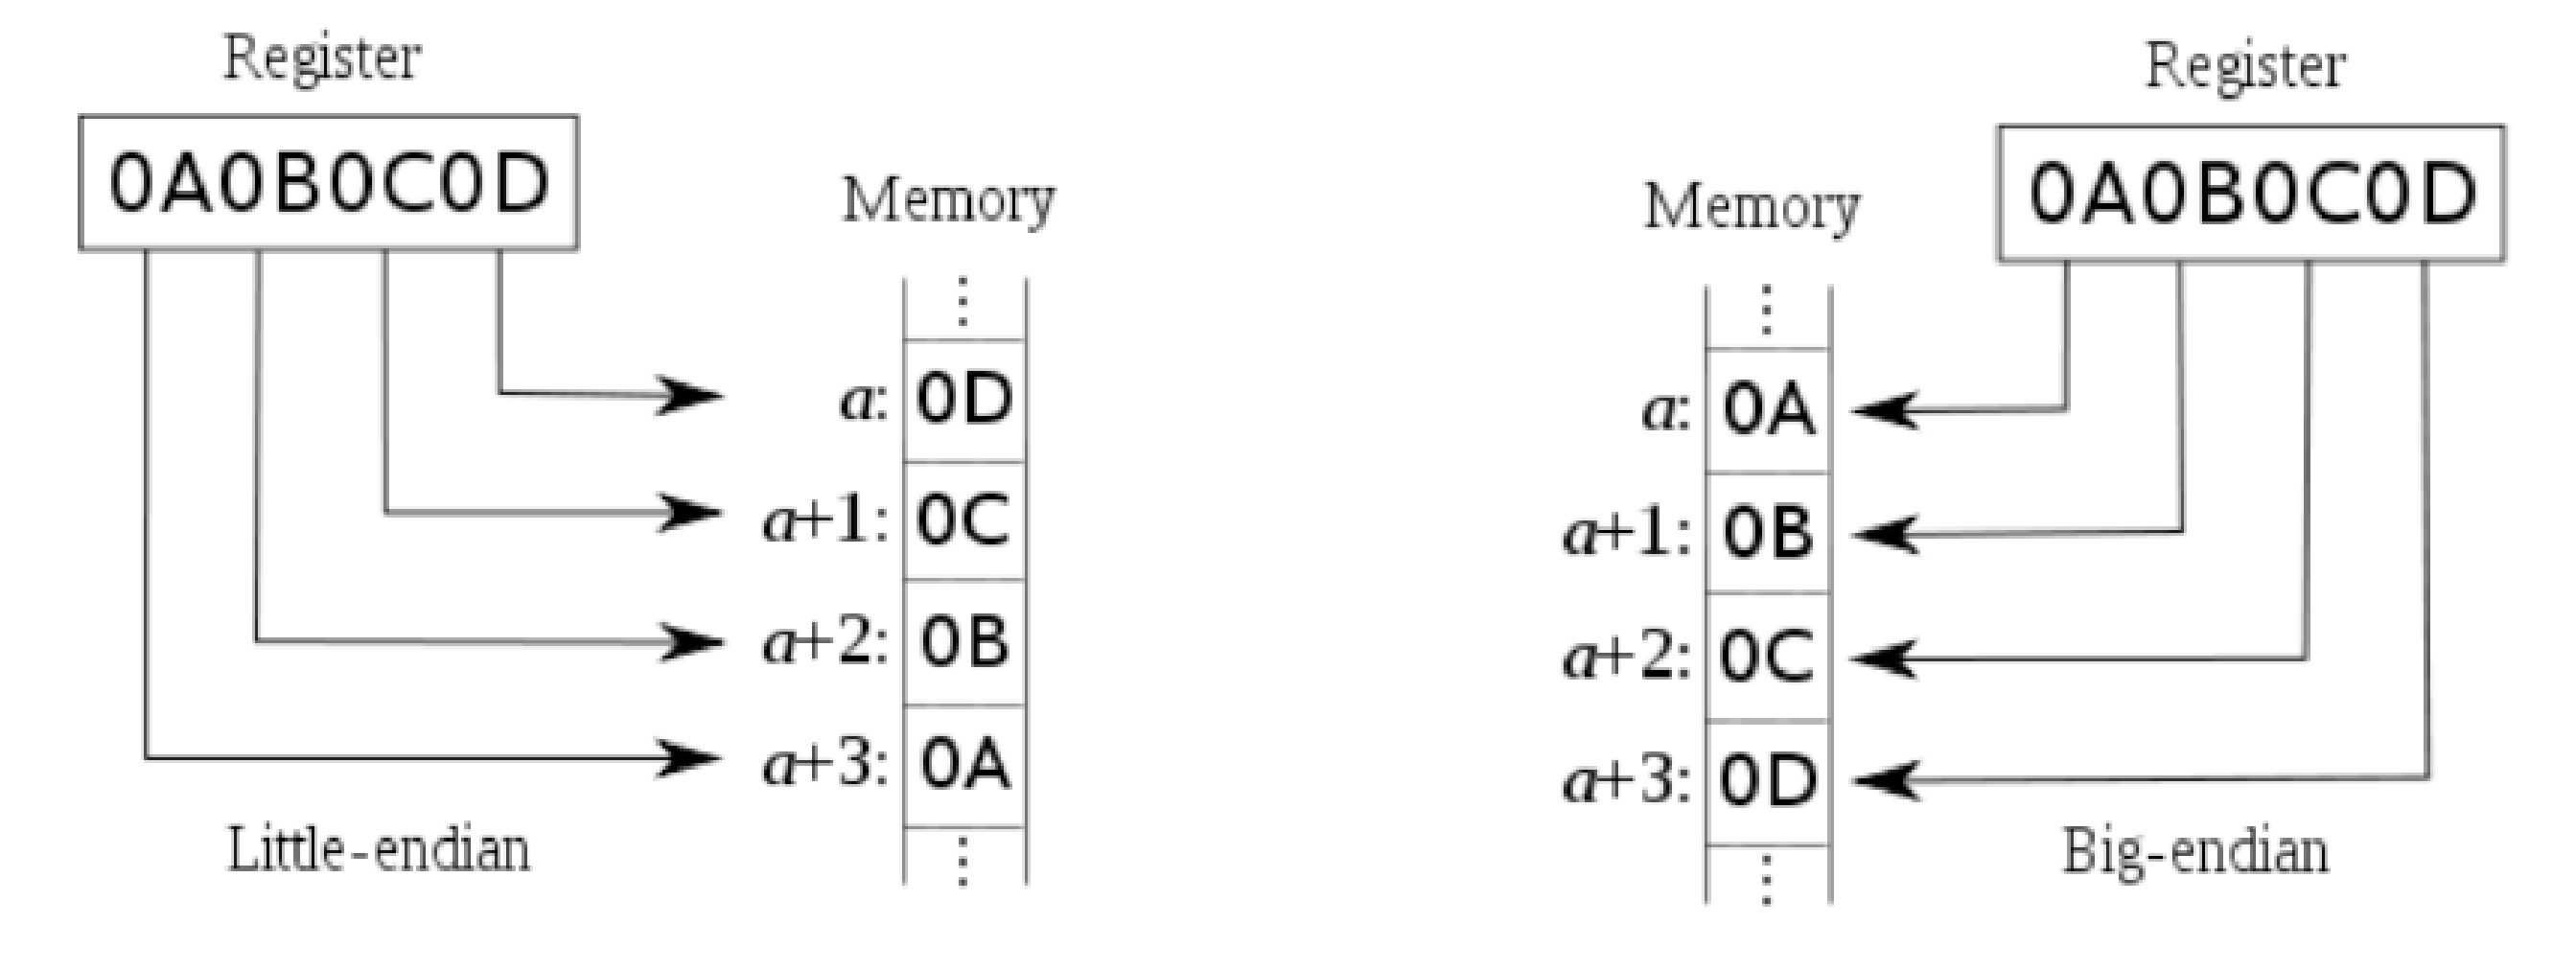
\includegraphics[width=11cm]{10_11}
\caption{Сравнение порядков от младшего к старшему и от старшего к младшему}
\end{figure}